\documentclass[conference]{IEEEtran}
\usepackage[T1]{fontenc}
\usepackage{cite}
\usepackage{booktabs}
\usepackage{tabularx}
\usepackage{amsmath}
\usepackage{tikz}
\usetikzlibrary{arrows.meta,positioning}
\usepackage[hidelinks]{hyperref}
\urlstyle{same}
\hypersetup{pdftitle={TripyTravy: Design and Evaluation of a Local-First Travel Itinerary Delivery System},pdfauthor={Unman Chaudhuri}}

\title{TripyTravy: Design and Evaluation of a Local-First Travel Itinerary Delivery System}
\author{
\IEEEauthorblockN{Unman Chaudhuri}
\IEEEauthorblockA{\textit{Department of Computer Science and Engineering}\\
\textit{Institute of Engineering \& Management Kolkata}\\
Kolkata, West Bengal, India}
\and
\IEEEauthorblockN{Coauthor 1 \quad Coauthor 2 \quad Coauthor 3}
% Replace these labels with confirmed names and affiliations before submission.
}


\begin{document}
\maketitle
\begin{abstract}
TripyTravy is a local-first travel itinerary system for agent authoring and traveler access. Its stable design combines a desktop Creator, a mobile Viewer, and a versioned \texttt{.tt} file containing schedules, locations, and supporting material. The agent can password-protect a transfer and change that password through a new export. The Viewer unlocks each protected package at import and opens the saved itinerary without a password prompt. The paper traces trip, day, event, location, image, and document workflows on both sides and compares them with Travefy's documented features. The evaluation uses the available beta implementation. A probe migrated an existing Kashmir itinerary and preserved checklist state. In a controlled test, eight references to one 1 MiB attachment produced a package 87.5\% smaller than eight distinct attachments of equal size. The beta wrapper accepted a modified metadata byte. The stable design uses authenticated encryption from a standalone Rust prototype whose application integration remains to be evaluated.
\end{abstract}

\begin{IEEEkeywords}
travel itinerary authoring, local-first software, offline import, versioned snapshots, content-addressed storage
\end{IEEEkeywords}

\section{Introduction}
A traveler may need both the time of a hotel check-in and the voucher for it. When an agent changes either one, the traveler needs the revised itinerary and a way to tell it from the copy already saved. A hosted link can point to the latest version. The traveler still needs to receive the update before going offline.

The agent edits a trip in the desktop Creator and sends a file containing the schedule, attachments, and revision information through a channel such as email. Once the file is on the traveler's device, the mobile Viewer can import it and open the saved copy from local storage. Neither operation requires a TripyTravy service.

Each trip has one publisher. The Creator holds the editable itinerary, and the Viewer keeps the most recent accepted snapshot it has received. Travelers can change their own checklists and completion status locally. Those changes stay on the traveler's device. In this paper, decentralized delivery means exchanging itinerary files without a central itinerary server.

We describe how TripyTravy protects files with a passphrase and replaces a saved schedule while preserving traveler state. We evaluate revision handling, package size, and malformed inputs across several beta builds. We also report separate tests of the Rust prototype and describe the remaining stable-release workflows. The comparison with Travefy follows the same tasks from scheduling an event to opening a voucher during a trip.

\section{Literature Review}
\label{sec:literature}

\subsection{Trip planning and information in the field}
Brown and Chalmers used field observations and diaries to study how tourists combine information sources while moving through a city \cite{brown}. Their findings motivate placing the day's plan and its tickets in one artifact. The GUIDE system provides a different kind of mobile help. Cheverst \emph{et al.} used visitor and environmental context to tailor a city guide \cite{guide}. TripyTravy's traveler app presents the schedule and places chosen by the agent. It can open a destination on a map, and the underlying itinerary stays available as a local record.

Several studies address the earlier task of deciding where to go. Gavalas \emph{et al.} classify problem formulations that combine a set of attractions with time and traveler constraints \cite{ttdp}. The City Trip Planner chooses and orders attractions across a plan with visit times and opening hours \cite{city}. De Choudhury \emph{et al.} derive candidate routes from geotagged photo traces \cite{breadcrumbs}. Lim \emph{et al.} estimate interests and visit durations from travel sequences and use them to recommend tours \cite{perstour}. Adamo \emph{et al.} also account for travel mode, linking a road tour with pedestrian subtours from parking locations \cite{multimodal}. These works distinguish automatic route generation from a delivery system for booked or manually chosen events. In TripyTravy, dates, durations, meeting points, and transport details come from the author. A map handoff keeps the event order and delegates navigation.

\subsection{Offline records and update semantics}
Local-first software connects device-local work to data ownership and offline access \cite{localfirst}. Coda demonstrates disconnected work through caching and reintegration when the server becomes reachable \cite{coda}. TripyTravy receives local data from an explicitly transferred snapshot, so its reader has no server reintegration step.

Bayou handles independent writes with dependency checks and application-specific merge procedures \cite{bayou}. Dynamo combines object versioning with reconciliation for replicas that can diverge \cite{dynamo}. Conflict-free replicated data types give convergence conditions for replicated writes \cite{crdt}. Unison formally specifies file synchronization using a common baseline and two replica states \cite{unison}. TripyTravy's editable trip has one publishing workflow, so a monotonic counter orders its exports and the mobile schedule requires no two-way merge. This counter is independent of both the device's wall clock and event times. Lamport's distinction between event ordering and physical time provides the broader systems context \cite{lamport}. The closer application precedent is iCalendar's \texttt{UID} and \texttt{SEQUENCE}, which let a client identify and reschedule the same event \cite{itip}.

\subsection{Storage and security}
Venti uses content fingerprints to share duplicate blocks in archival storage \cite{venti}. TripyTravy applies content addressing at whole-attachment granularity. The Low-Bandwidth File System avoids retransmitting matching chunks across files and versions \cite{lbfs}. TripyTravy's export savings concern duplication within a single package. The agent sends a complete snapshot on each revision. Results on crash-consistent applications show why validation of a staged file replacement alone cannot establish recovery across several persisted records \cite{crash}.

Saltzer and Schroeder's open-design and least-privilege principles distinguish format recognition from access control \cite{saltzer}. Felt \emph{et al.} show how permissions used by Android code can be studied separately from the data it processes \cite{permissions}. The Viewer uses an Android URI grant when passing an attachment to a document app. That grant controls access to the selected local file. Update authenticity remains a package-level problem. Samuel \emph{et al.} study signing roles and key compromise in update systems \cite{tuf}, while Mercury studies the bandwidth costs of authenticated rollback protection \cite{mercury}. A revision check in TripyTravy rejects previously seen older exports under normal use. Its current wrapper provides no authenticated origin. Argon2 research addresses the computational cost of password guessing \cite{argon} and informs the separate native prototype, whose integration status is described in Section~\ref{sec:container}.

\subsection{Travel software and scope of comparison}
KDE Itinerary supports whole-trip export and can suggest an existing trip when a ticket arrives \cite{kde}. Travefy provides a commercial reference for agent authoring and client delivery \cite{travefybuilder}. Its hosted link reflects edits when the traveler opens or refreshes it \cite{travefyupdates}. The mobile app also offers offline download \cite{travefyoffline}. These capabilities motivate comparing when each traveler receives the itinerary and how later revisions reach the device. Section~\ref{sec:comparison} compares those workflows using vendor documentation.

\section{Methodology}
\label{sec:methodology}

\subsection{Literature and feature evidence}
The study pairs a requirements-based specification of the stable release with source analysis and measurements from the available beta. The stable workflows are drawn from the project requirements, architecture specification, and the specified transfer-password lifecycle. The literature review focused on the functions and design decisions in those workflows. Searches combined terms for tourist trip design, mobile guides, disconnected replicas, content-addressed storage, filesystem persistence, and secure updates. Twenty-one journal or conference papers and one university research report were analyzed. For each work, the review recorded the method or finding and the specific TripyTravy claim it supports or bounds. Author copies and publisher records were used where available. The bibliography includes product manuals and standards as separate supporting sources.

For the feature analysis, the application entry points and the paths they call were traced from authoring through storage, export, import, and presentation. Desktop records were checked against their mapped \texttt{TripPackage} fields to distinguish available inputs from what the mobile reader receives. The Android manifest and Kotlin activity establish the intended platform handoffs. The Dart adapter wired into each application establishes the active container design. The independent Rust code and its tests establish the prototype design. Travefy features were checked against its public builder guide and help articles. This reflects documented Travefy behavior. It provides no account-level test or view of the vendor's implementation.

\subsection{Functional tests and controlled fixtures}
The evaluation ran on Windows 11 with Flutter 3.47.7 and Dart 3.13.5. The tested code was based on commit \texttt{65db5df} with the revision changes included in the accompanying patch. The desktop and mobile Flutter suites ran on the host. Native build artifacts came from the Windows Creator and Android Viewer. The study gathered no build or runtime data for macOS, Linux, or iOS. The Dart core tests used generated trips and local repositories, and the Rust tests exercised the native container in isolation.

A standalone Dart probe used a fresh disk-backed repository to import a legacy Kashmir export. It checked an item on the local checklist, exported a revised trip with a permanent ID, and imported the revision. It asserted that one trip remained, its title reflected the revision, and the checklist item stayed checked. The probe reopened the original file and checked that the newer revision remained current.

For the size test, the probe generated two, four, or eight distinct document records with 1 MiB payloads. Within each pair, the shared case reused exactly the same payload, and the distinct case varied its first byte for each record. Trip and document fields were held constant except for values derived from the bytes. The probe measured the final package length and asserted that the intended record and unique-blob counts survived import. A separate wrapper test packed a small JSON object, mutated one payload byte, and checked whether decoding accepted the changed object.

\section{Technology Stack and Target Platforms}
\label{sec:stack}
The desktop Creator and mobile Viewer use Flutter and Dart. The Creator targets Windows, macOS, and Linux, and the Viewer targets Android and iOS. Flutter supports native deployment on each platform \cite{flutterplatforms}. Both apps use \texttt{tripytravy\_core} for the trip model, attachment indexing, and the codec that writes and reads protected files. Protobuf metadata, Drift/SQLite for mobile records, and MapLibre rendering remain options for the stable design. Table~\ref{tab:stack} lists the components used in the evaluation.

\begin{table}[t]
\caption{Implementation stack}
\label{tab:stack}
\centering
\small
\renewcommand{\arraystretch}{1.12}
\begin{tabularx}{\columnwidth}{@{}>{\raggedright\arraybackslash}p{0.26\columnwidth}>{\raggedright\arraybackslash}X@{}}
\toprule
Component & Technologies and role \\
\midrule
Applications & Flutter and Dart for authoring, import, schedule viewing, and checklist operations. \\
Desktop storage & SQLite through \texttt{sqflite\_common\_ffi}. File picker, clipboard, and application-directory plugins support local authoring. \\
Mobile storage & JSON records and content-addressed files using Dart file I/O and plugin-provided application directories. \\
Shared exchange & Dart serialization, \texttt{crypto} for SHA-256, and a passphrase-protected binary container with UTF-8 JSON metadata. \\
Native runners & Windows C++ and CMake. Android Kotlin and Gradle with Flutter platform channels. \\
Native prototype & Rust and Cargo with AES-GCM, Zstandard, HKDF, and Argon2id. Evaluated separately from the Dart application codec. \\
\bottomrule
\end{tabularx}
\end{table}

The desktop code initializes SQLite, finds application support directories, and selects a command to open the export location on Windows, macOS, and Linux. The evaluation used the Windows Creator and Android Viewer runners. It gathered no build or runtime data for macOS, Linux, or iOS. An iOS build could reuse the Dart import and viewing code and would need counterparts for the Kotlin file receipt, document opening, and map handlers in Section~\ref{sec:native}.

\section{Authoring and Traveler Workflows}
\label{sec:features}

\subsection{Creator workspace and trip lifecycle}
The Creator opens a local trip library. An agent selects a trip or creates one with a title, date range, description, and banner. The stable design adds destination tags, a primary IANA time zone, currency, language, and a local traveler directory. An agent can keep contact, dietary, emergency, and passport-expiry information in that directory. The Creator compares the passport expiry date with the trip end date and flags validity under six months for the agent to review. The trip view exposes day schedules and a separate Information and Documents area. The agent can find exported copies in a library of timestamped files. The editable workspace remains distinct from those exports.

Trip dates supply the initial sequence of day records. Each day belongs to the trip and has its own date, title, and ordered events. In the evaluated Creator, extending the date range adds days. Shortening it removes empty days beyond the new range and retains days containing events. The stable Creator places the trip and day navigator beside the timeline and uses an inspector for the selected event or route. Moving a card across days changes its day association. The scheduler sorts timed cards by start time and uses display order for ties. It converts each timestamp to an instant using its recorded IANA zone. Two timed events overlap when each begins before the other ends. The agent sees a conflict and can adjust the relevant card in the inspector. Untimed notes retain a display position. Flight departure and arrival each carry their own time zone. The beta allows day reordering, but its export mapper defaults event time zones to UTC and can supply default times for untimed records.

\subsection{Typed event cards}
An event card gives an agent an editing surface and a traveler a summary of what to do. The stable data model assigns each event an identifier, a day, a display order, and a type. The renderer selects the fields appropriate to the type and resolves optional attachments through the asset index. The six cases below describe the intended fields and actions. The beta has typed card groups and a partial mapping into these records.

\begin{itemize}
\item \emph{Flight}. The agent enters the airline, flight number, airports, local departure and arrival times, terminals, seats, baggage, and reference number. The traveler sees both ends of the journey and can open the linked boarding pass or copy the booking reference.
\item \emph{Lodging}. The agent records check-in and check-out, property contacts, room and meal details, and confirmation. The traveler can see the property on a map, call it, or open its voucher and photos.
\item \emph{Transportation}. The agent chooses a mode and enters carrier, pickup and drop-off, coach or seat, and instructions. The traveler sees the pickup point and time next to the ticket. The beta retains display subcategories, while part of its structured transport mapping defaults to driving.
\item \emph{Activity}. The card holds the meeting point, start time, duration, operator, and instructions. The traveler can open the location or ticket from the card.
\item \emph{Dining}. The card holds the restaurant, reservation time, cuisine or dietary notes, and any menu or reservation file. Its location opens through the map action.
\item \emph{Information and advisory}. A note carries formatted instructions with an optional category, severity, checklist, or supporting file. Examples include visa reminders, packing instructions, and emergency contacts.
\end{itemize}

\subsection{Location cards and navigation}
The Creator can attach more than one location card to an event. A transfer can have separate pickup and drop-off cards. The parser extracts a name and coordinates where possible. Short links may require a redirect lookup. Missing coordinates or place names may trigger a Nominatim request. Each saved card retains the available name, coordinate pair, and map URL.

The beta Viewer opens a saved map link or creates a place search from a coordinate pair or name. For a day route, it traverses events in display order and collects one query per usable location card. It removes consecutive duplicate queries. A single stop opens a search. Two or more stops become the origin, destination, and intervening waypoints in a Google Maps directions URL \cite{maps}. This workflow delegates route computation to the map provider.

The stable Creator walks the day's ordered stops to build route connectors between consecutive locations. The agent can request an online ground route or supply manual or geodesic geometry for a leg. Each connector records its endpoints, mode, encoded polyline, distance, and duration. The agent can also draw an area or add a point of interest with opening hours and notes. The Viewer filters connectors, numbered stops, attraction pins, and polygons by the selected day. MapLibre draws these overlays above a basemap and an optional PMTiles street slice. Selecting a route focuses it on the map. Selecting an attraction opens its details. Embedded tiles and saved geometry support local display during the trip.

\subsection{Images, documents, and information}
The agent can add a trip banner, place event photos through the file picker or clipboard, and attach documents to either an event or an entry in Information and Documents. The two document entry points support different tasks. A rail ticket belongs beside its departure event. General instructions and emergency contacts belong at trip level. The editor stores description formatting with the record, so the Viewer can reconstruct headings, lists, and inline emphasis from serialized text. Rendering parity for every desktop control has yet to be evaluated.

The beta workspace and exporter can deduplicate identical documents and photos by hashing their bytes. Records can retain separate titles and filenames while sharing a stored blob. The exporter embeds readable local assets and records their digest, offset, and byte length. A banner can travel in its own field. Some external image URLs remain links, and a document whose source file is missing can retain metadata without usable bytes. The exporter also prepends synthesized note events for certain trip-level document records. The stable design keeps trip-level material in its own collection and renders it independently of the scheduled cards.

The Viewer resolves an embedded image by its asset reference and displays it in a swipeable, zoomable gallery. A document card resolves the corresponding bytes and opens the selected file. The beta can hand a temporary local copy to an installed Android handler. The stable Creator resizes eligible photos to a 1,920-pixel maximum edge and encodes them as WebP or JPEG before hashing the packaged bytes. Ticket and barcode legibility constrains that conversion. The Viewer looks up the asset by digest and sends the bytes to the offline gallery or PDF reader. The PDF reader exposes page thumbnails and zoom for vouchers or instructions. The size experiment measures exact-byte deduplication in the beta.

\subsection{Viewer library and day navigation}
The Viewer opens the local trip library without a sign-in step. It imports a package from the file picker or a supported operating-system file-open action. A newly accepted itinerary appears in the local trip library. The traveler opens a trip, selects a day, and can swipe between days or select an event from the day index to scroll to that card. In the stable Viewer, selecting a day scrolls the timeline to its first card. Scrolling across a day boundary updates the selected day. The timeline labels times in each event's recorded zone and opens a card's location, photos, or documents in a dedicated view. Trip-wide material remains accessible from Information and Documents. The Viewer renders the schedule in read-only mode. Checking a packing item changes its local state against the trip and item identifiers. Schedule replacement preserves those records and the trip's completion status. The stable Viewer displays a container integrity indicator after envelope and asset checks complete. The beta supports active and completed views and lets the traveler restore a completed trip to the active list.

\subsection{Stable delivery options}
The stable Creator offers a printable PDF with the day schedule, booking references, and emergency contacts. It also offers editable templates alongside ordinary and password-protected exports. The template compiler removes traveler records, booking references, and private vouchers before packaging the remaining data. Reusing a template starts a new editable trip with its own identifier. The distribution portal publishes app downloads, release checksums, and a gallery of sanitized templates. Private trip delivery uses the agent's chosen transfer channel. Its roadmap also includes a browser Viewer, an anonymous release feed, tablet authoring, and direct local transfer. These capabilities define the wider product design. The experiments in this paper use the native Creator and Viewer code paths and the shared Dart core.

\section{Functional Comparison with Travefy}
\label{sec:comparison}
Both products cover the agent's initial trip outline through the traveler's use of a scheduled item. We compared the TripyTravy beta with Travefy's documented workflows in Table~\ref{tab:features}. Section~\ref{sec:features} describes the additional stable workflows.

\begin{table*}[t]
\caption{Documented itinerary workflows and implementation boundaries}
\label{tab:features}
\centering
\small
\renewcommand{\arraystretch}{1.16}
\begin{tabularx}{\textwidth}{@{}>{\raggedright\arraybackslash}p{0.18\textwidth}*{2}{>{\raggedright\arraybackslash}X}@{}}
\toprule
Operation & TripyTravy & Travefy \\
\midrule
Create a trip and organize days &
Edit a local trip with date-range days and manual day ordering. &
Build a day-based itinerary. Events can be moved between days \cite{travefybuilder,travefymove}. \\
Add scheduled events &
Create typed cards and enter dates, times, location, and event details in the desktop workspace. &
Add scheduled places and activities with time and timezone fields. Type-specific tools include flight lookup and lodging check-in and check-out entries \cite{travefytime,travefyflight,travefylodging}. \\
Add trip guidance and supporting files &
Attach notes, event photos, and documents to the itinerary. Local embedded assets are indexed by digest on export. &
Add general trip information and attach documents at the trip or event level. An advisor can add images and videos to events \cite{travefyinfo,travefyfiles,travefymedia}. \\
Use itinerary locations &
Store place data and send a saved place or ordered day stops to Google Maps. &
Display places with addresses on the itinerary map \cite{travefymap}. \\
Share and read &
Send a passphrase-protected \texttt{.tt} snapshot. The traveler unlocks it at import and can later open the locally saved schedule and bundled assets. &
Share a web link, invitation, or PDF. Trip Plans can save the trip on a device. Its traveler account is optional for basic viewing \cite{travefyshare,travefyapp}. \\
Issue and receive a revision &
Export the edited itinerary again and send the new file. The receiver applies the newer matching revision on import. &
Edit the hosted itinerary. A shared web link reflects the revision when opened or refreshed \cite{travefyupdates}. \\
Prepare for offline travel &
Transfer the file before leaving connectivity or obtain it by direct transfer. External map and media URLs still use external services. &
Use the offline download workflow. Travefy advises opening items and attachments online to ensure the required data is available \cite{travefyoffline}. \\
\bottomrule
\end{tabularx}
\end{table*}

In either product, an agent can schedule a hotel arrival and attach its voucher. TripyTravy stores that information in SQLite and writes it to the trip package on export. Travefy hosts the itinerary and documents tools for importing supplier content and reusing library entries \cite{travefybuilder}. In TripyTravy the agent enters flight details. Travefy documents a lookup that populates a flight event \cite{travefyflight}. These form fields alone do not establish a live feed of booking updates.

Travefy includes its advisor tools in a subscription with other business functions \cite{travefypricing}. TripyTravy's evaluated exchange works without an account service or a hosted itinerary record. Each TripyTravy file carries its own copy of the schedule. A Travefy link points to the current hosted version, and travelers can download a copy for offline reading.

\section{System Architecture}
\label{sec:architecture}

\begin{figure}[t]
\centering
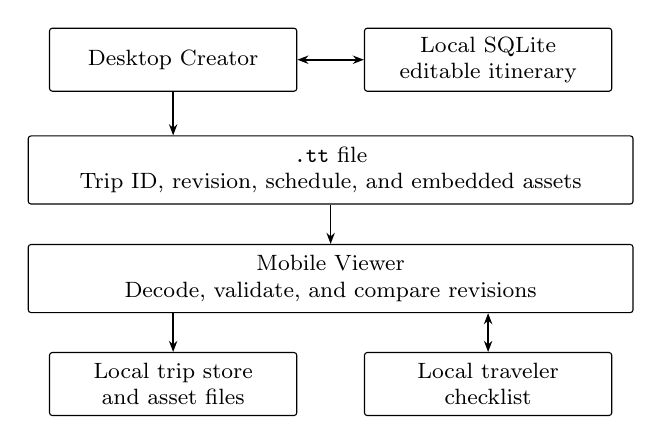
\begin{tikzpicture}[
  component/.style={draw, rounded corners=1pt, align=center,
    minimum height=8mm, text width=30mm, inner sep=2pt, font=\footnotesize},
  transfer/.style={draw, rounded corners=1pt, align=center,
    text width=74mm, inner sep=4pt, font=\footnotesize},
  flow/.style={-{Stealth[length=4pt]}, semithick},
  both/.style={{Stealth[length=4pt]}-{Stealth[length=4pt]}, semithick}]
  \node[component] (author) at (-20mm,0) {Desktop Creator};
  \node[component] (sqlite) at (20mm,0) {Local SQLite\\editable itinerary};
  \node[transfer] (file) at (0,-14mm) {\texttt{.tt} file\\Trip ID, revision, schedule, and embedded assets};
  \node[transfer,below=5mm of file] (viewer) {Mobile Viewer\\Decode, validate, and compare revisions};
  \node[component] (records) at ([xshift=-20mm,yshift=-9mm]viewer.south) {Local trip store\\and asset files};
  \node[component] (check) at ([xshift=20mm,yshift=-9mm]viewer.south) {Local traveler\\checklist};
  \draw[both] (author) -- (sqlite);
  \draw[flow] (author.south) -- (author.south |- file.north);
  \draw[flow] (file) -- (viewer);
  \draw[flow] (viewer.south -| records.north) -- (records.north);
  \draw[both] (viewer.south -| check.north) -- (check.north);
\end{tikzpicture}

\caption{The Creator publishes a snapshot. The Viewer stores the imported itinerary and traveler checklist in separate local records.}
\label{fig:delivery}
\end{figure}

\subsection{Shared core and storage}
Both apps use the Dart core for the trip model, file codec, and import and export operations. The core defines ports for storage and the codec \cite{hex}. Desktop screens also call SQLite directly for routine editing. On Android, the shared importer saves trips and checklist records as JSON and keeps binary assets in a file store (Fig.~\ref{fig:delivery}).

The stable design calls for transactional Drift/SQLite storage in the Viewer and atomic asset writes. The importer would validate and stage assets before publishing the schedule. Its transaction would preserve the checklist and carry forward the completion state. Once the traveler receives a file, the exchange can proceed without a server or analytics service. Download, messaging, routing, and map services have their own network requirements.

\subsection{Attachment indexing}
The exporter hashes document and event-photo bytes with SHA-256 \cite{sha}. Records that refer to identical bytes can point to one blob. Each asset descriptor gives its digest, size, and offset in the attachment region. For versioned exports, the importer checks attachment bounds and verifies the hashes of all indexed assets. The mobile store names each asset file by its digest. A re-export can index legacy inline data. The banner has its own field and is outside the size experiment in Section~\ref{sec:evaluation}.

\section{Revision Handling}
\subsection{Identity and export ordering}
The Creator allocates a 128-bit random identifier in SQLite when a trip is first exported by the versioned path. It encodes the value as 32 hexadecimal digits with a \texttt{tt\_} prefix. The database stores it with a revision counter. The export path reserves the next revision in a database transaction before compiling the file. A failed export can leave a gap in the sequence. A title change has no effect on the trip identifier.

\subsection{Acceptance and replacement}
For a versioned import, let $i$ denote the trip identifier and $r$ the incoming revision. Let $r_s$ be the saved revision for $i$ when a versioned entry exists. The beta runs the revision decision after decoding and asset validation. The stable protected path also requires successful envelope authentication before comparing revisions. The service applies the following rule.
\begin{equation}
\operatorname{decision}(i,r)=
\begin{cases}
\text{create}, & \text{no matching entry},\\
\text{replace}, & r>r_s,\\
\text{keep saved}, & r\leq r_s.
\end{cases}
\label{eq:revisions}
\end{equation}
The Flutter file picker and Android file-open route reach the same import service. Imports through one service instance are queued, so simultaneous submissions do not interleave the revision decisions. The repository writes the accepted trip to a staging file and renames it into the trip's local path. A successful replacement writes a complete snapshot into the existing entry. The accepted snapshot occupies the existing itinerary entry, and the replaced snapshot is discarded from the trip library. The checklist remains a separate record under the same identifier, and the importer copies the local completion flag into the accepted snapshot. The original file may still exist in the transfer application or Downloads.

\subsection{Migration from numeric identifiers}
Earlier exports exposed a numeric SQLite row ID, which could coincide across separate Creator databases. For migration, a versioned package carries that former ID. The Viewer requires a matching numeric ID and at least one shared event identifier before migrating a saved legacy entry. It transfers the checklist, preserves completion state, saves the versioned record, and removes the migrated legacy entry. If the legacy trip and incoming snapshot have no event in common, the Viewer cannot establish that correspondence and saves the versioned trip separately. The revision rule in (\ref{eq:revisions}) applies directly once the permanent identifier is in use.

\section{Native Integration}
\label{sec:native}

\subsection{Windows and Android integration in the beta}
The Windows application uses a native SQLite library through the Dart FFI adapter for editing and export metadata. File-picker and clipboard integrations bring local files into the workspace. The export path can save a copy using the platform save dialog and reveal the resulting file through Windows Explorer. This leaves distribution to the agent's chosen transfer channel.

On Android, the Kotlin activity accepts a matching \texttt{ACTION\_VIEW} intent. It reads the associated URI through Android's content resolver. The activity buffers bytes for an initial launch and forwards subsequent intents over the Flutter method channel. The Dart import service also accepts files from the application's file picker. Both binary entry paths use the same decoder and repository logic.

Document opening reverses the handoff. The application resolves the local attachment, supplies a content URI through Android's \texttt{FileProvider}, and launches an \texttt{ACTION\_VIEW} chooser with a read grant \cite{provider}. The receiving application needs to handle the given file type. For a map request the activity targets Google Maps first, then falls back to another registered handler if needed. File association, local document access, and map dispatch are separate native operations.

\subsection{Stable file receipt}
The stable Viewer sends picker and system-open requests to the same validation pipeline. A share provider can supply a content stream whose URI lacks a filename extension. On Android, the handler can query the provider's display name and inspect the first four bytes for the \texttt{TTRV} marker. The name and marker identify candidates. The decoder checks the full envelope before accepting a package. The iOS target needs the corresponding Files and share-sheet integration. The stable design also specifies a browser-based Viewer for local import. Cross-platform build, file association, and offline runtime behavior remain to be validated.

\section{The \texttt{.tt} Container and Security Design}
\label{sec:container}

\subsection{Snapshot structure and compatibility}
A \texttt{.tt} file contains the complete itinerary and its embedded attachments. The Creator assigns the trip ID and revision, serializes the itinerary as JSON in the protected beta, and includes one copy of each distinct attachment. The Viewer selects a decoder by format and version. It can still read supported legacy files, which should be treated as unprotected. The Creator writes every new export in the passphrase-protected format. If authentication fails, the Viewer ends that import attempt. It uses the legacy decoder only for files it identifies as legacy.

\subsection{Authenticated encryption in the applications}
Both apps use the same Dart codec. On each export, the Creator requires a passphrase and generates a random salt and nonce. Argon2id and HKDF-SHA256 derive a key from the passphrase and salt \cite{argonrfc,hkdfrfc}. AES-256-GCM encrypts the itinerary metadata and attachments and authenticates the header \cite{gcm}. The Viewer uses the received salt and the entered passphrase to derive the key, then verifies the envelope before parsing the metadata. The filename remains visible. The codec limits the protected payload to 64 MiB and runs key derivation and encryption outside the interface isolate.

The earlier Rust prototype tested authenticated packing and compression on its own. The apps now use the Dart codec, and the size experiment measures the savings from storing one copy of each distinct attachment.

\subsection{Password lifecycle in the stable design}
\label{sec:password}
Only the Creator workspace exposes controls for setting or changing an itinerary password. The agent sets the password for a trip and sends the protected export to the intended travelers. The agent can communicate the password separately from the file. A traveler may enter the password to open a received package. The Viewer has no control for setting the password, changing it, or publishing a replacement export.

A password change is a publishing operation. The Creator retains the trip identifier, reserves a higher revision, generates a fresh salt and nonce, and encrypts a new snapshot using the new password. This applies even when the schedule is identical. The Creator may then distribute the new file through the same channel as the original. Password protection belongs to each exported file. Earlier files still use their original passwords. A traveler can keep reading the schedule already saved on the device.

At import, the Viewer reads the format and checks bit 2 of the native envelope's flags to decide whether to prompt. An import cancelled at the prompt leaves the library as it was. The import path checks framing and length before prompting. The flag becomes authenticated only after the GCM tag verifies. For a protected file, the Viewer holds the supplied password for key derivation and uses the salt and nonce carried in that file. If authentication fails, the Viewer reports the unlock failure and leaves the existing itinerary intact. After successful authentication, the Viewer decompresses and validates the snapshot, checks the trip ID and revision, and stores a new trip or replaces the matching saved version. A stale or equal revision does not replace the saved schedule. Replacement preserves the checklist and completion flag.

The import password is needed again for a later protected package, even when that package updates a trip already on the phone. For a password-only revision, the traveler enters the new password at import. The old password will not unlock the newly encrypted file. Once the new version is saved, the traveler reads it from local storage without an itinerary-password prompt. The Viewer discards the transfer password and derived key after use. Operating-system and storage controls govern access to the extracted files.

For example, an agent issues Kashmir revision 3 with password A, then changes the password and sends revision 4 with password B. A traveler who already imported revision 3 can continue reading it. The Viewer asks for B when opening revision 4. After validating the package, it updates the one locally saved Kashmir trip. Subsequent access to that saved trip needs neither A nor B. The example describes the expected behavior of the stable design.

The shared password grants access to anyone who learns it. A short PIN remains guessable offline despite the cost of Argon2id. The Creator's exclusive editing controls belong to the application interface. To establish that a revision came from the original agent, the Viewer would need a trusted publisher key and a signature covering the trip identifier, revision, and package contents. The standard mode derives its key from a common seed that can be recovered from the software.


\subsection{Validation and publication to local storage}
Before asking for a passphrase, the reader checks the file framing and protected payload size. After authentication, it checks the trip ID and revision, verifies attachment extents and digests, and checks that each protected record points to an included asset. It finishes those checks before writing assets or saving the trip. Legacy imports also undergo identity, bounds, and storage-key checks. The Viewer records whether a saved trip came from an authenticated transfer so it can reject a newer unprotected replacement. Recovery from an interruption between asset, schedule, and traveler-state writes still needs device testing.

\section{Results}
\label{sec:evaluation}
These results describe the evaluated beta paths and the separately tested Rust library. The end-to-end transfer-password workflow and the five-attempt policy are stable design specifications.

\subsection{Functional and revision tests}
The desktop suite passed 52 tests, the mobile suite passed 23, and the Dart core passed 13. A separate three-test Rust suite checked round-trip packing, PIN handling, and authenticated header tamper rejection for the native prototype. Those Rust results concern the isolated library.

The desktop tests cover date-based records, event and document persistence, description formatting, image-upload controls, and export naming and metadata. The mobile tests cover picker import, day navigation, photo-gallery behavior, document presentation, and the ordered map URL. These tests exercise application logic and widgets. The Android platform handoffs were verified by source inspection.

The revision tests submit multiple imports to the same service instance, including a newer snapshot followed by earlier files. The repository retains the newer revision and a single trip entry. The tests also cover separate entries for unrelated itineraries with the same legacy number, and rejection of a non-versioned identifier carrying a positive revision. The desktop export test inspects the emitted identifier and verifies that the next reservation advances its revision.

The probe imported an existing 2,638,655-byte Kashmir export and marked one packing item complete. It then exported a modified copy with the permanent identifier, a revised title, and revision~1. After import, the repository contained one trip with the revised title and one completed checklist item. Reopening the original file left revision~1 in place. This probe exercises the file-based client core. The application suites separately exercise the desktop export control and mobile file-picker path.

\subsection{Package size}
All document records survived export and import. Table~\ref{tab:dedup} reports the package sizes. The reduction in total package bytes is $100(1-B_s/B_d)$ percent, where $B_s$ and $B_d$ are the measured package sizes with shared and distinct payloads, respectively.

\begin{table}[t]
\caption{Export size for equal-length document payloads}
\label{tab:dedup}
\centering
\small
\begin{tabular}{rrrr}
\toprule
References & Shared (B) & Distinct (B) & Reduction \\
\midrule
2 & 1,049,768 & 2,098,680 & 50.0\% \\
4 & 1,050,196 & 4,196,932 & 75.0\% \\
8 & 1,051,052 & 8,393,436 & 87.5\% \\
\bottomrule
\end{tabular}
\end{table}

The shared-payload package grows by 1,284 bytes between two and eight references, because additional records add metadata without adding a second blob. The experiment measures byte equality in a controlled fixture. Savings for a real trip depend on how often passengers need the same attachment.

\subsection{Container mutation}
The probe packed a JSON object with the title \texttt{Trip A}. It changed the single wrapped byte for the final letter, then decoded the file without changing its trailer. The decoder returned \texttt{Trip B}. The test isolates the frame-level check and shows that it accepts altered metadata. Hash checks on assets do not cover that field.

\section{Discussion}
\subsection{Who owns the schedule and when it changes}
A traveler can receive a new TripyTravy snapshot through an existing transfer channel and import it after going offline. This avoids a dependency on a vendor itinerary service during import. It also gives the agent responsibility for redistributing each revision and the traveler responsibility for opening it. Revision comparison orders the files the traveler has already received. It cannot tell the traveler that an unseen revision exists.

The entire snapshot can initialize a new device. Repeated attachments inside one export occupy one blob per distinct payload, and an existing blob may be reused on the recipient's device. Each file transfer still carries the packaged assets. The sender's messaging service, an external document viewer, and a map handoff have their own data and availability boundaries.

\subsection{Feature and evaluation limits}
The feature trace found gaps between the desktop forms and the serialized records, including default time zones and the loss of some transport modes during export. The stable workflows specify how those fields should reach the traveler's timeline. Template sanitization, embedded maps, and built-in offline PDF reading also sit outside the evaluated end-to-end paths.

The size experiment uses synthetic equal-length documents. Savings on a typical tour would depend on its media and the extent of document reuse. The repository and widget tests establish behavior for their test cases. Physical-device file delivery, airplane-mode operation, memory, latency, and crash recovery across trip and asset writes were outside the measured scope. The Travefy comparison uses public product documentation.

A forged beta metadata field could misstate the revision used for replacement. Authentication in the stable path checks that the envelope and payload are intact under the derived key. The shared password model leaves publisher identity unresolved, as Section~\ref{sec:password} describes.

Release validation for the protected workflow needs a full Creator-to-Viewer test. The critical cases are a first-time import, a cancel or incorrect password with an itinerary already saved, and a password-only revision that updates that itinerary in place. The test should also check that the earlier file cannot replace the newer saved revision and that the traveler can reopen the saved itinerary after restarting the app.

\section{Conclusion}
TripyTravy's stable design covers trip authoring, itinerary delivery, and reference material for offline travel. The Creator publishes a versioned snapshot, and the Viewer asks for a transfer password when opening a protected export. After import, the traveler reads the saved version directly from local storage. The beta evaluation established replacement and checklist preservation for the Kashmir fixture and measured the package savings from repeated attachments. The metadata mutation test makes authenticated import a prerequisite for trusting revision fields. The protected workflow and native platform handoffs require integrated release validation.

\begingroup
\raggedright
\IEEEtriggeratref{38}
\bibliographystyle{IEEEtran}
\bibliography{references,literature}
\endgroup
\end{document}
